%-----------------------------------------------------------------------------
% Author: Ramsey (Rayla) Phuc
% Alias: Rayla Kurosaki
% GitHub: https://github.com/rkp1503
%-----------------------------------------------------------------------------
\documentclass{rayla-project}
\usepackage{rayla-style}

%-----------------------------------------------------------------------------
% Project Information
%-----------------------------------------------------------------------------
\myUniversity{
    Rochester Institute of Technology\\
    College of Science\\
    School of Mathematical Sciences
    }
\myTitle{Red Blood Cell Production}
\myName{Ramsey (Rayla) Phuc}
\courseid{MATH-421.01}
\courseName{Mathematical Modeling}
\professorName{Dr. Nathan Cahill}
\term{2020/08/26 - 2020/11/24}
\dueDate{2020/12/07}

%-----------------------------------------------------------------------------
% Start of Document
%-----------------------------------------------------------------------------
\begin{document}

    \maketitle

    %-------------------------------------------------------------------------
    % Abstract
    %-------------------------------------------------------------------------
    \begin{abstract}
        Red Blood Cells are present in the human body and their purpose is to deliver oxygen to the human body while giving carbon dioxide for humans to exhale. The purpose of this paper is to show that Red Blood Cells can maintain an equilibrium state if a certain condition is met. Multiple models have been tested to show that this condition is consistent given the proper assumptions. The first model being analyzed is a system of linear difference equations. The second model being analyzed is a system of linear differential equations. The third model being analyzed is a system of nonlinear difference equations. This condition is where $\gamma = 1$.
    \end{abstract}

    %-------------------------------------------------------------------------
    % Body
    %-------------------------------------------------------------------------
    \section{Introduction and Background Information}
\label{sec:introduction-and-background-information}

Red Blood Cells are a type of cells that are present in the human body. They are red and the shape of a Red Blood Cell is like the shape of a donut but without a hole. In other words, a biconcave disc~\cite{article1}. Red Blood Cells are created through a process called erythropoiesis. It takes about a week for a Red Blood Cell to fully develop in the bone marrow and its life span is about four months~\cite{article2}. As humans inhale oxygen, the Red Blood Cells extract that oxygen and deliver it into the body. At the same time, the Red Blood Cells give carbon dioxide for humans to exhale~\cite{web1}.

    %-----------------------------------------------------------------------------
% Author: Ramsey (Rayla) Phuc
% Alias: Rayla Kurosaki
% GitHub: https://github.com/rkp1503
%-----------------------------------------------------------------------------
\section{Problem Statement}
\label{sec:problem-statement}

The circulatory system in the human body produces and destroys Red Blood Cells every day. The problem is to determine the number of Red Blood Cells on a particular day~\cite{book1}.

    \section{Initial Assumptions and Simplifications}
\label{sec:initial-assumptions-and-simplifications}

\begin{enumerate}
    \item Spleen filters out and destroys a certain fraction of the Red Blood Cells every day.
    \item Bone marrow produces a number of Red Blood Cells that is proportional to the number of Red Blood Cells lost on the day prior.
\end{enumerate}

    %-----------------------------------------------------------------------------
% Author: Ramsey (Rayla) Phuc
% Alias: Rayla Kurosaki
% GitHub: https://github.com/rkp1503
%-----------------------------------------------------------------------------
\section{Initial Conditions and Definitions}\label{sec:initial-conditions-and-definitions}

\begin{itemize}
    \item $n$ represents a particular day.
    \item $R_n$ represents the number of Red Blood Cells circulating in the blood on day $n$.
    \item $M_n$ represents the number of Red Blood Cells produced by the bone marrow on day $n$.
    \item $f$ represents the fraction of Red Blood Cells the spleen removes.
    \item $\gamma$ represents the number of Red Blood Cells produced per number of Red Blood Cells lost.
\end{itemize}

    \section{Mathematical Methods}
\label{sec:mathematical-methods}

\subsection{Model 1}
\label{subsec:model-1}

In this model, we will solve the problem through a discrete approach using Linear Difference Equations.

\subsubsection{Building the Model}

For a particular day $n$, we can define the number of Red Blood Cells that is present in the blood for the next day $R_{n+1}$ as follows. We reduce the number of Red Blood Cells by a particular factor $(1-f)$ to represent the number of Red Blood Cells lost on day $n$ and we add the number of Red Blood Cells the bone marrow produces on day $n$.\\

Also for a particular day $n$, we can define the number of Red Blood Cells the bone marrow produces on the next day $M_{n+1}$ as follows. The number of Red Blood Cells produced is proportional to the number of Red Blood Cells present in the blood $R_n$ with a factor of $\gamma f$ where $\gamma f$ represents the proportionality constant of the production of Red Blood Cells.\\

Based on the given initial assumptions and simplifications as well as the initial conditions, we can create a system of linear difference equations.

\begin{equation}
    \begin{dcases}
        R_{n+1} &= (1-f)R_n + M_n\\
        M_{n+1} &= \gamma fR_n
    \end{dcases}
    \label{eq:linear-difference-model-system}
\end{equation}

\subsubsection{Analysis: Equilibrium}

Instead of using a system of linear difference equations, we can use a higher-order homogeneous linear difference equation. From \myref[Equation]{eq:linear-difference-model-system}, we can use the expression of $M_{n+1}$ and substitute it into the expression of $R_{n+1}$, giving us:

\begin{equation}
    R_{n+1} =  (1-f)R_n + \gamma fR_{n-1}
    \label{eq:linear-difference-model-equation}
\end{equation}

Lets denote $R_{n+1} = g(R_n)$.
If we assume that there exists a $\bar{R}$ such that the Red Blood Cell count remains in an equilibrium state, then we can say that

\[
\bar{R} = \lim_{n\to\infty} R_{n+1} = \lim_{n\to\infty} g(R_n) = g\left(\lim_{n\to\infty} R_n\right) = g(\bar{R}).
\]

From this, we can solve for $\bar{R}$:

\begin{align}
    \bar{R} &= (1-f)\bar{R} + \gamma f\bar{R} \nonumber\\
    0 &= \bar{R}[(1-f) + \gamma f - 1] \nonumber \\ 
    \implies \bar{R} &= 0 \label{eq:R-bar-value}
\end{align}

This value of $\bar{R}$ is the particular solution to our difference equation and is not that interesting because this value of $\bar{R}$ tells us that a possible equilibrium state is where there are no Red Blood Cells present in the human body. \\

What is interesting is the values of $f$ and $\gamma$ from \myref[Equation]{eq:R-bar-value}. Assuming that $\bar{R} \neq 0$, then we can derive the following expression:

\begin{align} 
    0 &= \bar{R}[(1-f) + \gamma f - 1] \nonumber\\
    0 &= (1-f) + \gamma f - 1 \nonumber\\
    0 &= -f + \gamma f \nonumber\\
    0 &= f(\gamma - 1), \label{eq:parameter-values}
\end{align}

where \myref[Equation]{eq:parameter-values} yields $f=0$ and $\gamma=1$. Here, we can ignore this value of $f$. This is because this value of $f$ implies that in order to maintain a constant production of Red Blood Cells in the body, the spleen must not remove any Red Blood Cells. This result implies a few contradictions. For starters, this contradicts our first initial assumption where we assumed that the spleen filters out and destroys a certain amount of Red Blood Cells every day. This also contradicts the fact that if the spleen does not filter out and destroy Red Blood Cells, then the number of Red Blood Cells will continue to increase without a limit. Thus, we can assume that $f\neq0$.\\

However, this value of $\gamma$ is significant. This would imply that to maintain an equilibrium of Red Blood Cells in the human body, the spleen must produce one Red Blood Cell for each one destroyed. This makes sense since adding a Red Blood Cell after removing a Red Blood Cell should not impact the equilibrium state drastically. With further analysis, we can confirm this value of $\gamma$. To do this, we can rewrite \myref[Equation]{eq:linear-difference-model-equation} in the following form:

\begin{equation}
    R_{n+1} - (1-f)R_n - \gamma fR_{n-1} = 0
    \label{eq:linear-difference-model-equation-2}
\end{equation}

which shows that \myref[Equation]{eq:linear-difference-model-equation-2} is a homogeneous equation. Thus, the complementary solution is in the form of:

\begin{equation*}
    R_n = c_1\lambda_1^n + c_2\lambda_2^n
\end{equation*}

where $c_1,c_2$ are constants. To find these lambda values, we will solve the following characteristic equation:

\begin{equation}
    \lambda^2 - (1 - f)\lambda - \gamma f = 0
    \label{eq:linear-difference-model-characteristic-equation}
\end{equation}

Solving \myref[Equation]{eq:linear-difference-model-characteristic-equation} for $\lambda$ using the quadratic formula yields the following values of $\lambda$:

\[
\begin{dcases}
    \lambda_1 &= \frac{1-f + \sqrt{(1-f)^2 + 4\gamma f}}{2}\\
    \lambda_2 &= \frac{1-f - \sqrt{(1-f)^2 + 4\gamma f}}{2}
\end{dcases}
\]

Using these expressions for $\lambda$, we will show that the total number of Red Blood Cells that is present in the blood will remain constant under a specific condition. Let $\lambda_1=1$. Then we have:

\begin{align*}
    \lambda_1 &= \frac{1-f + \sqrt{(1-f)^2 + 4\gamma f}}{2}\\
    1 &= \frac{1-f + \sqrt{(1-f)^2 + 4\gamma f}}{2}\\
    2 &= 1-f + \sqrt{1 - 2f + f^2 + 4\gamma f}\\
    1 + f &= \sqrt{1 - 2f + f^2 + 4\gamma f}\\
    (1 + f)^2 &= 1 - 2f + f^2 + 4\gamma f\\
    f^2 + 2f + 1 &= 1 - 2f + f^2 + 4\gamma f\\
    4f &= 4\gamma f\\
    \implies\gamma &= 1.
\end{align*}

This implies that to maintain an equilibrium of Red Blood Cells in the human body, we need the condition where $\gamma = 1$, which is exactly what we found earlier. Using this result, we can determine the value of $\lambda_2$:

\begin{align*}
    \lambda_2 &= \frac{1-f - \sqrt{(1-f)^2 + 4\gamma f}}{2}\\
    &= \frac{1-f - \sqrt{1-2f+f^2 + 4(1)f}}{2}\\
    &= \frac{1-f - \sqrt{f^2+2f+1}}{2}\\
    &= \frac{1-f - \sqrt{(f+1)^2}}{2}\\
    &= \frac{1-f - (f+1)}{2}\\
    &= \frac{-2f}{2}\\
    \lambda_2 &= -f.
\end{align*}

Knowing this value of $\lambda_2$, then we can say that the complementary solution is

\begin{equation} \label{eq:7}
    R_n = c_1(1)^n + c_2(-f)^n.
\end{equation}

% \begin{figure}[H] 
%     \centering
%     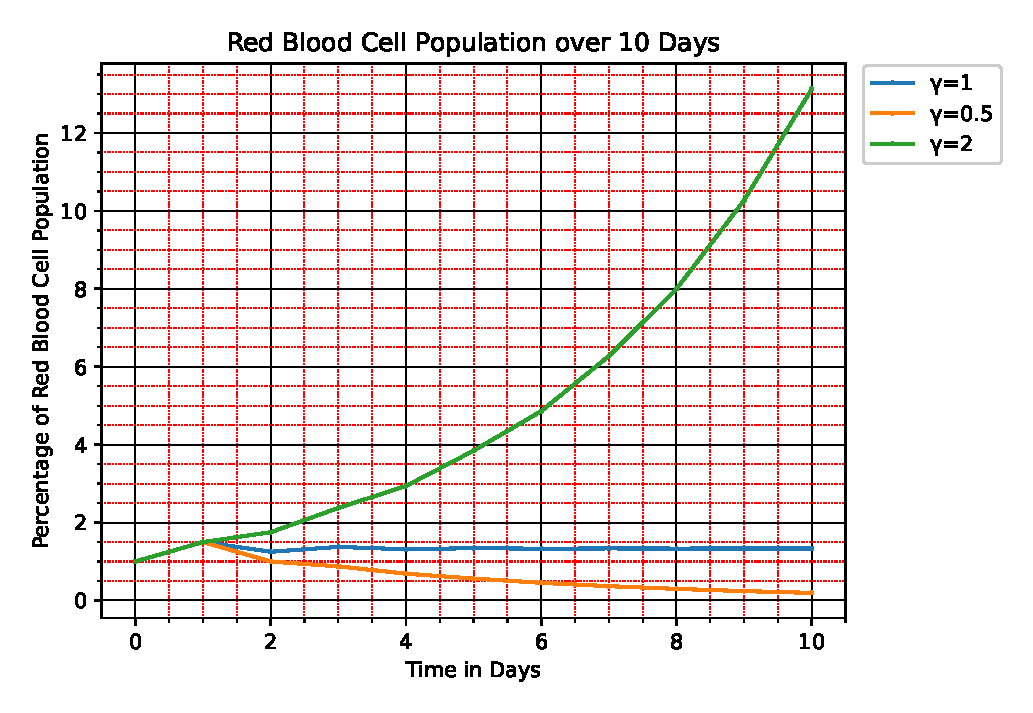
\includegraphics[width=0.5\textwidth]{Linear-Difference-Model.eps}
%     \caption{}
%     \label{fig:1}
% \end{figure}

\myref[Figure]{fig:1} displays the plots for the state of the population of Red Blood Cells $P_0$ with the parameters $f=0.5$ and different values of $\gamma$. For $\gamma=1$, we can see that the graph is constant, meaning that the Red Blood Cell population is in equilibrium. For other values of $\gamma$, this does not hold. In \myref[Figure]{fig:1}, we can see that for $\gamma = 0.5$, the number of Red Blood Cells will decrease and eventually go to 0. This shows that the population of Red Blood Cells will converge to 0 as $n\to\infty$ for $\gamma < 1$. In \myref[Figure]{fig:1}, we can see that for $\gamma = 2$, the number of Red Blood Cells will increase without an upper bound. This shows that the population of Red Blood Cells will increase continuously as $n\to\infty$ for $\gamma > 1$.

\subsection{Model 2}
\label{subsec:model-2}

In this model, we will solve the problem through a continuous approach using ordinary differential equations using Model 1 as a base.

\subsubsection{Building the Model}

To create this model, we will start with \myref[System]{eq:linear-difference-model-system} and convert that to a system of ordinary differential equations. We will start by converting the first equation in \myref[System]{eq:linear-difference-model-system}. We can rewrite that equation in the following form:

\begin{equation*}
    R_{n+1} - R_n = M_n - fR_n
\end{equation*}

We know that dividing an expression by 1 does not change the expression. So we can divide the left hand side by $n+1-n$:

\begin{equation*}
    \frac{R_{n+1} - R_n}{(n+1)-n} = M_n - fR_n
\end{equation*}

Here $n$ is a discrete time variable where $n$ is the number of days. We will change our initial assumption of $n$ by letting $n$ be a continuous time variable. Now, instead of determining the number of Red Blood Cells in the $n+1$ day, we will consider the number of Red Blood Cells in the $n+\Delta n$ day. This changes the equation to:

\begin{equation*}
    \frac{R_{n+\Delta n} - R_n}{(n+\Delta n)-n} = M_n - fR_n
\end{equation*}

Then, we can rewrite it in a way such that both $R$ and $M$ are functions of time. Therefore, with a change of variables, we obtain:

\begin{equation*}
    \frac{R(t+\Delta t) - R(t)}{(t+\Delta t)-t} = M(t) - fR(t)
\end{equation*}

We can simplify the left hand side and notice that if we take the limit as $\Delta t\to\infty$, we have the definition of the derivative. Thus applying that limit to both sides yields:

\begin{align}
    \lim_{\Delta t\to\infty} \frac{R(t+\Delta t) - R(t)}{\Delta t} &= \lim_{\Delta t\to\infty} (M(t) - fR(t)) \nonumber\\
    R'(t) &= M(t) - fR(t) \label{eq:linear-differential-equation-R}
\end{align}

We will convert the second equation in \myref[System]{eq:linear-difference-model-system} in a similar manner. We will first subtract $M_n$ on both sides:

\begin{equation*}
    M_{n+1} - M_n = \gamma fR_n - M_n
\end{equation*}

Then we will divide the left hand side by $(n+1)-n$.

\begin{equation*}
    \frac{M_{n+1} - M_n}{(n+1)-n} = \gamma fR_n - M_n
\end{equation*}

Then, we will use the new assumption that $n$ is now a continuous time variable. We will now consider the number of Red Blood Cells produced on day $n+\Delta n$. Thus, with a change of variables and letting $R$ and $M$ be functions of time, we have:

\begin{equation*}
    \frac{M(t+\Delta t) - M(t)}{(t+\Delta t)-t} = \gamma fR(t) - M(t)
\end{equation*}

If we take the limit as $t\to\infty$, we have:

\begin{align} 
    \lim_{\Delta t \to\infty}\frac{M(t+\Delta t) - M(t)}{(t+\Delta t)-t} &= \lim_{\Delta t \to\infty} (\gamma fR(t) - M(t)) \nonumber\\
    M'(t) &= \gamma fR(t) - M(t).\label{eq:linear-differential-equation-M}
\end{align}

Therefore, with \myref[Equation]{eq:linear-differential-equation-R} and \myref[Equation]{eq:linear-differential-equation-M}, our system of differential equations are:

\begin{equation}
    \begin{dcases}
        R'(t) &= M(t) - fR(t)\\
        M'(t) &= \gamma fR(t) - M(t)
    \end{dcases}
    \label{eq:linear-differential-model-system}
\end{equation}

\subsubsection{Analysis: Equilibrium}

We will determine the equilibrium state of the population of Red Blood Cells. Here, the trivial case is where there are no Red Blood Cells present in the human body. Thus, we can say that $R'(t) = 0$ and $M'(t) = 0$. This, of course, is not an interesting solution. But we can use this information to determine other potential equilibrium state(s). If we took the limit as $t\to\infty$, then we can say that $R(t) = R^\ast(t)$ and $M(t) = M^\ast(t)$. Thus, we have the system of differential equations to solve:

\begin{equation*}
    \begin{dcases}
        0 &= M^\ast(t)-fR^\ast(t)\\
        0 &= \gamma fR^\ast(t) - M^\ast(t)
    \end{dcases}
\end{equation*}

From this set of equations, we can deduce that

\begin{align*}
    M^\ast(t) &= fR^\ast(t)\\
    M^\ast(t) &= \gamma fR^\ast(t)
\end{align*}

Since the left hand side of both equations are equivalent, then the equilibrium state of this system can only be achieved if $\gamma = 1$, which is what we concluded when analyzing the first model.

\subsection{Model 3}
\label{subsec:model-3}

In our initial assumptions, $f$ represents the number of Red Blood Cells removed by the spleen, and it is a constant fraction. Suppose that the spleen removes a fraction of Red Blood Cells that is dependent of the number of Red Blood Cells present in the human body. We would like to assume that if the number of Red Blood Cells increases, then the number of Red Blood Cells filtered out by the spleen will also increase non-linearly. If there is less Red Blood Cells present, then the number of Red Blood Cells filtered out will decrease non-linearly. In particular, lets assume that if there are no Red Blood Cells present, then $f=0$. If the number of Red Blood Cells is high enough, then $f \approx 1$. With this assumption of $f$, consider the following expression for $f$:

\begin{equation*}
    f(R_n) = 1 - \frac{1}{R_n+1}
\end{equation*}

This graph has a root at $R_n=0$ and it converges to 1 as $R_n\to\infty$ so it is suitable expression for $f(R_n)$.

\subsubsection{Building the Model}

With this new assumption, our system of equations becomes

\begin{equation}
    \begin{dcases}
        R_{n+1} &= \frac{R_n}{1 + R_n} + M_n\\
        M_{n+1} &= R_n\gamma-\frac{R_n\gamma}{1+R_n}
    \end{dcases}.
    \label{eq:nonlinear-difference-model-system}
\end{equation}

\subsubsection{Analysis: Equilibrium}

We can rewrite \myref[System]{eq:nonlinear-difference-model-system} as one, higher order, nonlinear difference equation.

\begin{equation}
    R_{n+1} = \frac{R_n}{1 + R_n} + R_{n-1}\gamma-\frac{R_{n-1}\gamma}{1+R_{n-1}}
    \label{eq:nonlinear-difference-model-equation}
\end{equation}

If we assumed that there exists an equilibrium state for the Red Blood Cell population $\bar{R}$, then:

\begin{align*}
     \bar{R} &= \frac{\bar{R}}{1 + \bar{R}} + \bar{R}\gamma - \frac{\bar{R}\gamma}{1+\bar{R}}\\
     1 &= \frac{1}{1 + \bar{R}} + \gamma - \frac{\gamma}{1+\bar{R}}\\
     1 + \bar{R} &= 1 + \gamma(1 + \bar{R}) - \gamma\\
     \bar{R} &= 1\gamma + \bar{R}\gamma - \gamma\\
     0 &= \bar{R}(1-\gamma)
\end{align*}

From this, we can conclude that the system will maintain an equilibrium state under two conditions. Both of which were present when we did a similar analysis on Model 1. We can rewrite \myref[Equation]{eq:nonlinear-difference-model-equation} in the following form of a homogeneous equation:

\begin{equation*}
    R_{n+1} - \frac{R_n}{1 + R_n} - R_{n-1}\gamma + \frac{R_{n-1}\gamma}{1+R_{n-1}} = 0
\end{equation*}

From the homogeneous equation, we can say that the characteristic equation is:

\begin{align}
    0 &= \lambda^2 - \frac{\lambda}{1 + \lambda} - \gamma + \frac{\gamma}{2} \nonumber\\
    0 &= 2\lambda^3+2\lambda^2-\lambda(\gamma+2)-\gamma. \label{eq:2nonlinear-difference-model-characteristic-equation}
\end{align}

Here, it will be difficult to find the analytic solution of $\lambda$. But we can still do analysis on it. If we let $\lambda = 1$, then we can conclude that

\begin{align}
    0 &= 2\lambda^3 + 2\lambda^2 - \lambda(\gamma + 2) - \gamma \nonumber\\
    0 &= 2(1)^3 + 2(1)^2 - (1)(\gamma+2) - \gamma \nonumber\\
    0 &= 2 + 2 - \gamma - 2 - \gamma \nonumber\\
    0 &= 2 - 2\gamma \nonumber\\
    \implies \gamma &= 1, \label{eq:nonlinear-difference-model-param-val}
\end{align}

which further supports the fact that $\gamma = 1$ is the condition where the number of Red Blood Cells in the human body will maintain in an equilibrium state. \myref[Figure]{fig:2} plots \myref[System]{eq:nonlinear-difference-model-system} for three different values of $\gamma$. Just like in Model 1, it is clear that the Red Blood Cell population will be in an equilibrium state when $\gamma = 1$, explode to infinity for $\gamma > 1$, and diminish to 0 for $\gamma < 1$.

    %-----------------------------------------------------------------------------
% Author: Ramsey (Rayla) Phuc
% Alias: Rayla Kurosaki
% GitHub: https://github.com/rkp1503
%-----------------------------------------------------------------------------
\section{Conclusion}
\label{sec:conclusion}

What we have done is shown that the only possible way for Red Blood Cell population to maintain in an equilibrium state is when $\gamma = 1$. An idea that can be extended from this work is to see what would happen if blood loss occurred at some day $n$ and how the state of the Red Blood Cell population would be affected if a small or a large portion of that population has been removed from the body.


    %-------------------------------------------------------------------------
    % Bibliography
    %-------------------------------------------------------------------------
    \newpage
    % \nocite{*}
    \printbibliography[title={Bibliography}]

    %-------------------------------------------------------------------------
    % Appendix
    %-------------------------------------------------------------------------
    \newpage
    \appendix
    \section{Figures}\label{sec:figures}

\begin{figure}[H] 
    \centering
    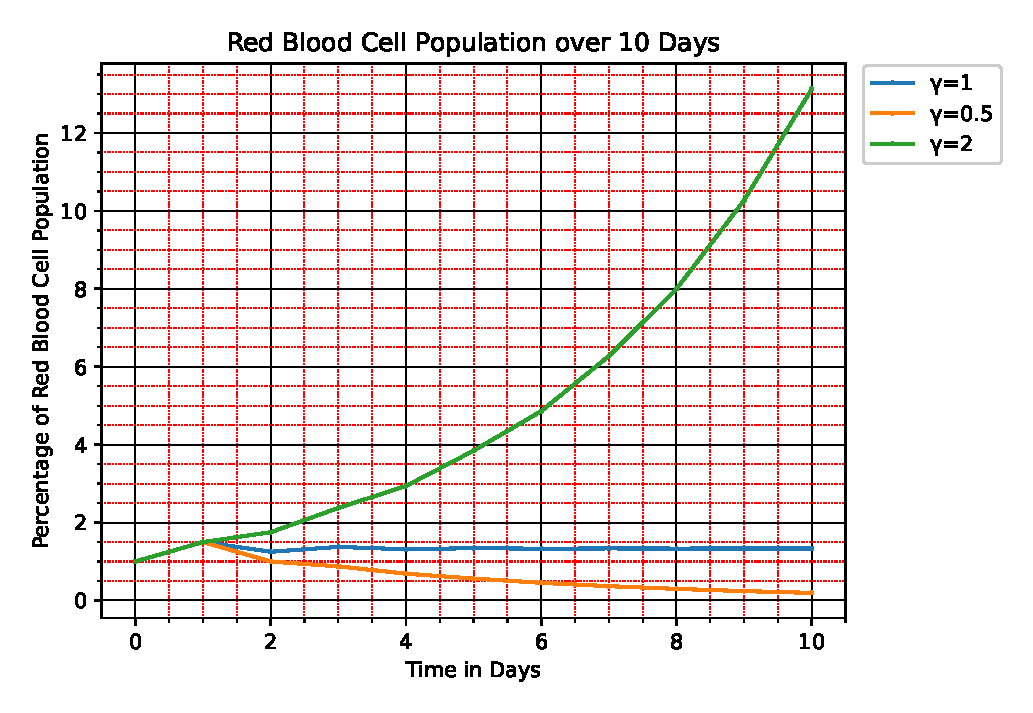
\includegraphics[width=0.81\textwidth]{Linear-Difference-Model.eps}
    \caption{A graph to numerically solve \myref[System]{eq:linear-difference-model-system} with initial conditions $R_0=100$, $M_0=100$, and $f=0.5$ for different value of $\gamma$ over $t=10$ days.}
    \label{fig:1}
\end{figure}

\begin{figure}[H] 
    \centering
    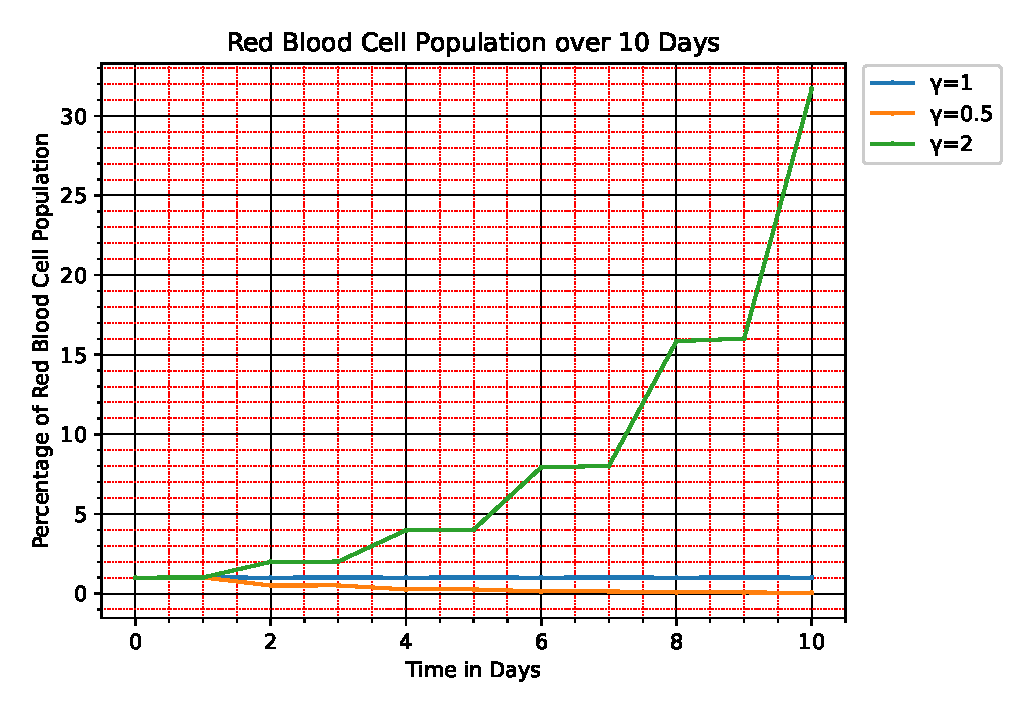
\includegraphics[width=0.81\textwidth]{Nonlinear-Difference-Model.eps}
    \caption{A graph to numerically solve \myref[System]{eq:nonlinear-difference-model-system} with initial conditions $R_0=100$, $M_0=100$, and $f=0.5$ for different value of $\gamma$ over $t=10$ days.}
    \label{fig:2}
\end{figure}

\end{document}
